\pagebreak
\section{Esperimenti e analisi dei risultati}

Il comando \textit{mmetric} ci permette di ottenere metriche e stime di performance sul nostro modello:
\begin{minted}{r}
metrics=mmetric(testset$shot_result,prediction,metric=c("ALL"))
\end{minted}

%TODO: aggiungere valori
\begin{table}[H]
\centering
  \begin{tabular}{l l} 
  Accuracy complessiva & xx\\
  Precision per la classe \textit{made} & xx\\
  Precision per la classe \textit{missed} & xx\\
  Recall per la classe \textit{made} & xx\\
  Recall per la classe \textit{missed} & xx\\
  F-measure per la classe \textit{made} & xx\\
  F-measure per la classe \textit{missed} & xx\\
  Area Under Curve complessiva & xx\\
    \end{tabular}
    \caption{Metriche del modello SVM}
\end{table}

\begin{table}[H]

%TODO: aggiungere valori
\centering
\noindent
\renewcommand\arraystretch{1.5}
\setlength\tabcolsep{0pt}
\begin{tabular}{c >{\bfseries}r @{\hspace{0.7em}}c @{\hspace{0.4em}}c @{\hspace{0.7em}}l}
\centering
  \multirow{10}{*}{\rotatebox{90}{\parbox{1.1cm}{\bfseries\centering Actual value}}} & 
    & \multicolumn{2}{c}{\bfseries Prediction outcome} & \\
  & & \bfseries p & \bfseries n & \bfseries total \\
  & p$'$ & \MyBox{True}{Positive} & \MyBox{False}{Negative} & P$'$ \\[2.4em]
  & n$'$ & \MyBox{False}{Positive} & \MyBox{True}{Negative} & N$'$ \\
  & total & P & N &
\end{tabular}
 \caption{Confusion Matrix di SVM}
 \label{confusion_matrix_svm}
\end{table}

L'esecuzione della Cross Validation non migliora molto questi risultati:

%TODO: aggiungere valori
\begin{table}[H]
\centering
  \begin{tabular}{l l} 
  Accuracy complessiva & xx\\
  Precision per la classe \textit{made} & xx\\
  Precision per la classe \textit{missed} & xx\\
  Recall per la classe \textit{made} & xx\\
  Recall per la classe \textit{missed} & xx\\
  F-measure per la classe \textit{made} & xx\\
  F-measure per la classe \textit{missed} & xx\\
  Area Under Curve complessiva & xx\\
    \end{tabular}
    \caption{Metriche risultate dell'esecuzione della cross validation su SVM}
\end{table}

\begin{table}[H]

%TODO: aggiungere valori
\centering
\noindent
\renewcommand\arraystretch{1.5}
\setlength\tabcolsep{0pt}
\begin{tabular}{c >{\bfseries}r @{\hspace{0.7em}}c @{\hspace{0.4em}}c @{\hspace{0.7em}}l}
\centering
  \multirow{10}{*}{\rotatebox{90}{\parbox{1.1cm}{\bfseries\centering Actual value}}} & 
    & \multicolumn{2}{c}{\bfseries Prediction outcome} & \\
  & & \bfseries p & \bfseries n & \bfseries total \\
  & p$'$ & \MyBox{True}{Positive} & \MyBox{False}{Negative} & P$'$ \\[2.4em]
  & n$'$ & \MyBox{False}{Positive} & \MyBox{True}{Negative} & N$'$ \\
  & total & P & N &
\end{tabular}
 \caption{Confusion Matrix di SVM dopo la cross validation}
 \label{confusion_matrix_svm_cv}
\end{table}

\begin{figure}[H]
  % QUA CI VA ROC PRIMA DI CV
  \centering
  \begin{subfigure}{.5\textwidth}
  \centering
  \caption{Prima}
  \label{roc-svm-missed-25k}
  \includegraphics[width=.8\linewidth]{roc-svm-missed-25k}
\end{subfigure}%
\begin{subfigure}{.5\textwidth}
  \centering
  \caption{Dopo}
  \label{roc-svm-made-25k}
  \includegraphics[width=.8\linewidth]{roc-svm-made-25k}
\end{subfigure}%
  \caption{ROC su SVM}
\end{figure}


Il risultato, intuitivamente un po' basso, è in realtà in linea con le aspettative: i fattori che influenzano un tiro a canestro sono molteplici, mentre le informazioni in nostro possesso sono limitate. Il fatto che sia comunque  superiore al \textit{random guessing} dimostra che esistono dei fattori nel dataset che tendono effettivamente ad influenzare il successo o il fallimento del tiro.

\par
% to do: verificare correttezza
Considerando la classe \textit{made} quella positiva e la classe \textit{missed} quella negativa, dalle metriche ottenute possiamo fare alcune valutazioni: per entrambe le classi il valore di precision è simile ed è sul 60\%, da cui deduciamo una proporzionalità di falsi positivi e falsi negativi.
Guardando le recall invece notiamo che per la classe \textit{missed} tendono ad esserci pochi falsi negativi, mentre la vera criticità è il numero eccessivo di falsi positivi per \textit{made}. In altre parole, un tiro legittimo tende ad essere considerato un fallimento.

Le F-measure sono valori che permettono di confrontare direttamente le due classi. Precision e recall sono spesso diverse e quindi è complicato determinare quale classe abbia effettivamente meno errori: la F-measure, ottenuta computando la media armonica di queste due metriche, permette di quantificare le performance delle due classi in maniera comparabile. Nel nostro caso era deducibile che la f-measure di \textit{missed} fosse molto più alta di quella di \textit{made}: la disparità nelle recall influisce molto sul calcolo complessivo.

Essendo un problema di apprendimento automatico binario, la Area Under Curve, intesa come AUROC (Area Under Receiver Operating Characteristic), è solo una. Tale metrica corrisponde all'area sottostante la ROC, ottenuta muovendo gradualmente la threshold della SVM e rappresentando sul grafo ogni volta i valori di TPR (\textit{True Positive Rate}) e FPR (\textit{False Positive Rate}).
Più grande (vicino a 1) è il valore della AUROC, più è grande la distinzione tra True Positive e True Negative: nel nostro caso vale 0,64.

\par
Sia eseguendo SVM sull'intero dataset, diviso opportunamente in training set (80\%) e trainset (il restante 20\%), sia eseguendolo con una 10-fold cross validation, il valore di accuracy complessivo tra le due esecuzioni non si discosta troppo. Ciò porta a concludere che il dataset è formato da istanze poco sofferenti di bias e difficilmente rischia di andare in overfitting.

\pagebreak
\subsection{Alberi di Decisione}
Per verificare come si comportassero altri modelli diversi dalla SVM, abbiamo dato in input il nostro dataset e abbiamo allenato un modello utilizzando gli alberi di decisione.
Innanzitutto è stata eseguita un'euristica per individuare il valore migliore di CP, ossia quello con \textit{xerror} minimo. Questo parametro indica di quanto debba migliorare il relative error complessivo per poter eseguire uno split nel nodo dell'albero.
Il risultato però è stato un albero con un solo split:

\begin{figure}[H]
\caption{Alberi di decisioni}
\label{dt_fig}
  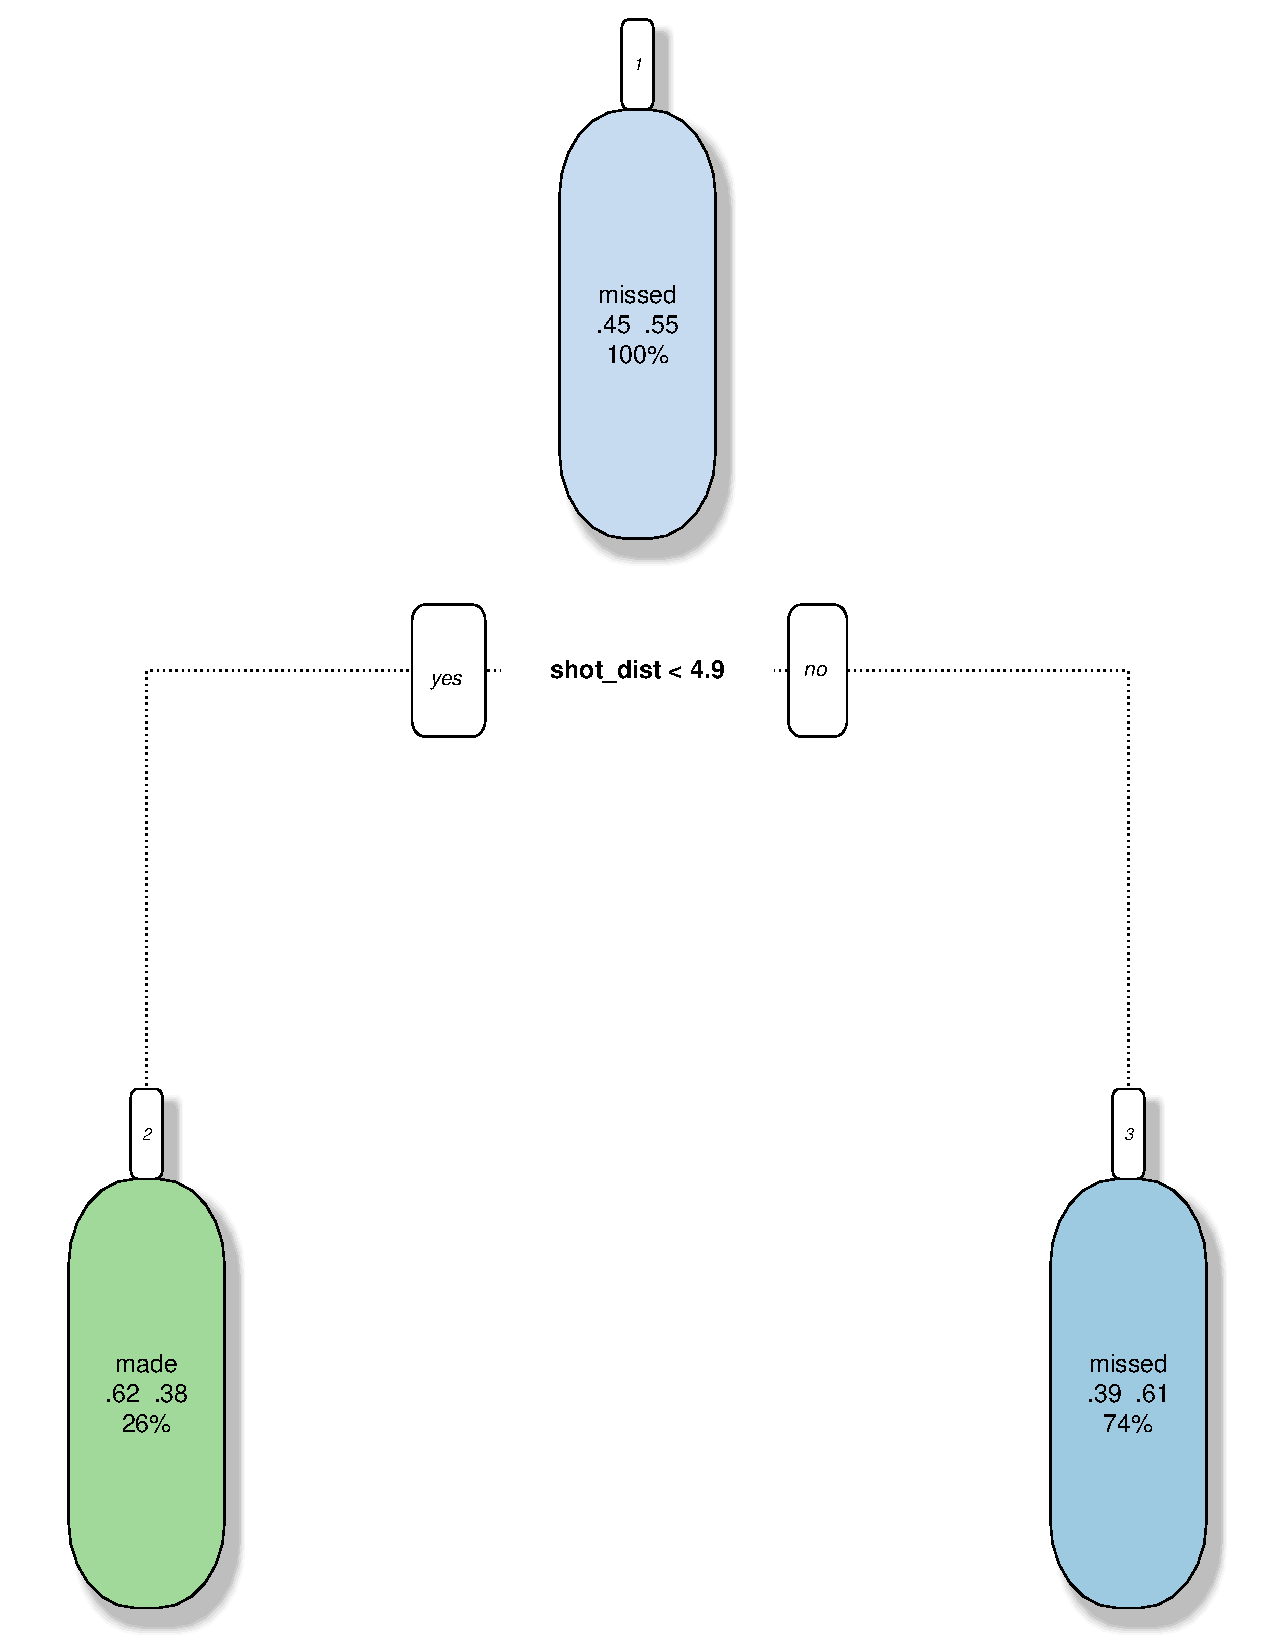
\includegraphics[width=\linewidth]{DECISIONTREE}
\end{figure}


Un'analisi delle metriche e del contributo informativo delle feature considerate ci mostra il perchè di un albero così corto:
\begin{table}[H]
\centering
  \begin{tabular}{l l} 
shot\_dist &77\\
shot\_clock &8\\
touch\_time &8\\
close\_def\_distance &7\\
percentage\_prev\_games &1\\
    \end{tabular}
    \caption{Importance in DT}
\end{table}

\begin{table}[h!]
\centering
  \begin{tabular}{l l} 
  Accuracy complessiva & 61.06\\
  Precision per la classe \textit{made} & 62.12\\
  Precision per la classe \textit{missed} & 60.68\\
  Recall per la classe \textit{made} & 35.71\\
  Recall per la classe \textit{missed} & 82.01\\
  F-measure per la classe \textit{made} & 45.35\\
  F-measure per la classe \textit{missed} & 69.75\\
    \end{tabular}
    \caption{Metriche risultate dell'esecuzione della cross validation su Decision Tree}
\end{table}

L'importance di \textit{shot\_dist} è nettamente più alta di qualsiasi altro attributo.
Questi valori dimostrano che il decision tree non è adeguato per il nostro problema in quanto non coinvolge attributi che per noi sono influenti e probabilmente generalizzerà male con istanze nuove.
Inoltre questo albero di decisione ottiene delle metriche peggiori della nostra SVM.

\begin{table}[H]

\centering
\noindent
\renewcommand\arraystretch{1.5}
\setlength\tabcolsep{0pt}
\begin{tabular}{c >{\bfseries}r @{\hspace{0.7em}}c @{\hspace{0.4em}}c @{\hspace{0.7em}}l}
\centering
  \multirow{10}{*}{\rotatebox{90}{\parbox{1.1cm}{\bfseries\centering Actual value}}} & 
    & \multicolumn{2}{c}{\bfseries Prediction outcome} & \\
  & & \bfseries p & \bfseries n & \bfseries total \\
  & p$'$ & \MyBox{20 639}{} & \MyBox{37 162}{} & P$'$ \\[2.4em]
  & n$'$ & \MyBox{12 587}{} & \MyBox{57 357}{} & N$'$ \\
  & total & P & N &
\end{tabular}
 \caption{Confusion Matrix di DT}
 \label{confusion_matrix_dt}
\end{table}